\documentclass{article}
\usepackage[utf8]{inputenc}
\usepackage[english]{babel}
\usepackage{graphicx}
\usepackage{float}
\usepackage{listings}

\title{Manual 1 - 2do Torneo de Programación Competitiva}
\author{Lions R.C.}
\date{Junio 2019}

\begin{document}

\maketitle

\begin{figure}[H]
    \centering
    
\includegraphics[width=0.2\paperwidth]{newblack}
\end{figure}

\section{Instalación de IDE para editar y compilar C++}

\subsection{Code::Blocks [Windows]}
Si desea instalar un programa para compilar codigo facilmente, puede descargar Code::Blocks de la pagina oficial: http://www.codeblocks.org/

Este programa permite al usuario escribir y compilar codigo en Windows sin tener que instalar las diversas herramientas de compilación a mano. Para descargarlo, debe ir a la sección de Downloads y escoger Binaries, y de ahi descargar cualquiera de las opciones que le aparece (le recomendamos la primera opción).

\begin{figure}[H]
    \centering
    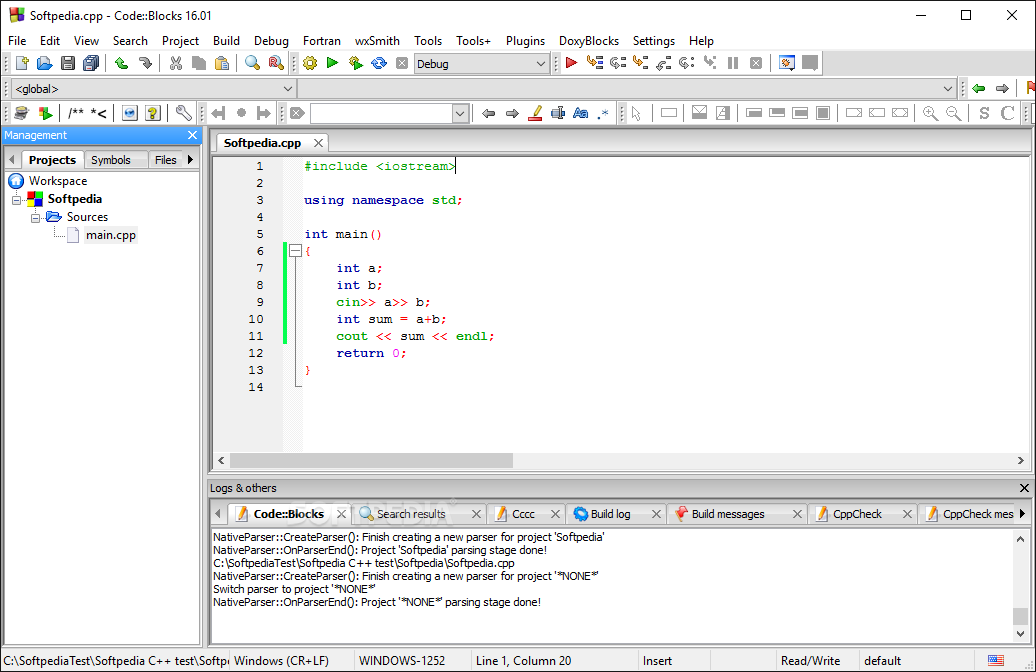
\includegraphics[width=0.5\paperwidth]{CodeBlocks}
\end{figure}

\subsection{Repl.it [Página web]}
Repl.it es una página web que te permite probar codigo desde cualquier plataforma, la unica desventaja puede ser que ocupes una cuenta para guardar tu código. Para usarlo, debe entrar a la página https://repl.it/languages/cpp

\begin{figure}[H]
    \centering
    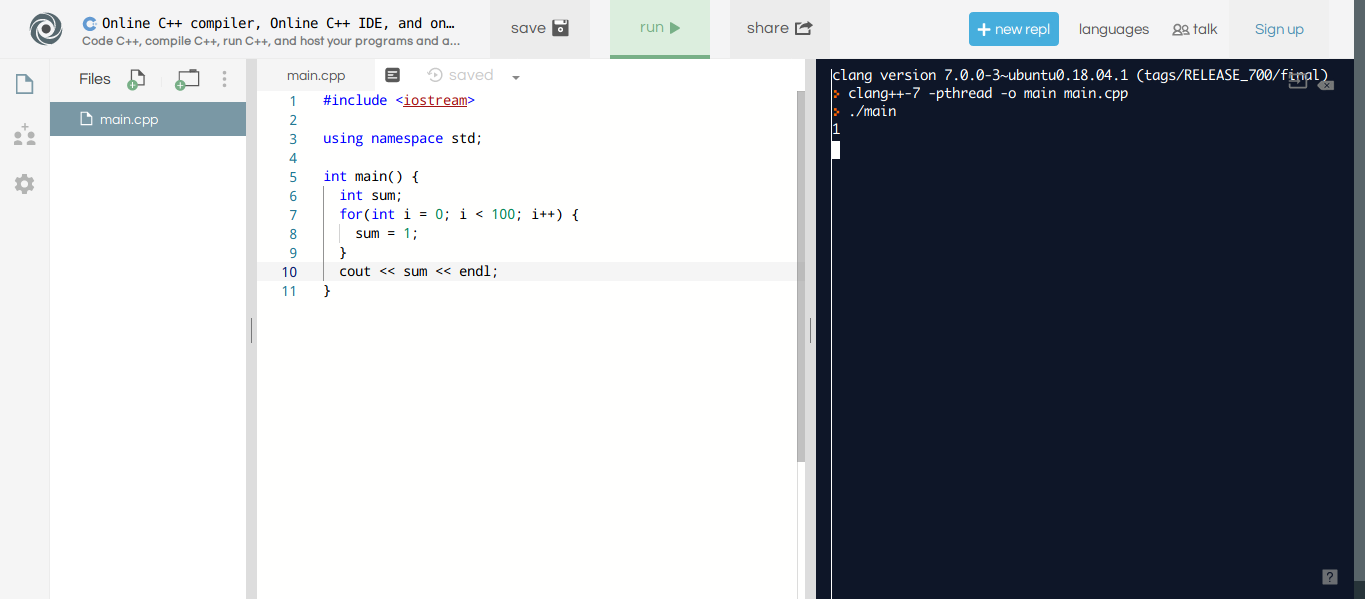
\includegraphics[width=0.5\paperwidth]{replit}
\end{figure}

\subsection{Visual Studio Community [Windows y Mac]}
Esta es la versión gratis del software famoso de Microsoft llamado Visual Studio, te permite compilar código en muchos lenguajes y ofrece herramientas avanzadas de analisis de código.

Se puede descargar en la página oficial https://visualstudio.microsoft.com/vs/community/ y te permite usarlo siempre y cuando estes ingresado con una cuenta de Microsoft. Si no tiene una cuenta de Microsoft y quisiera utilizar este programa, puede registrarse uno en https://account.microsoft.com/account?lang=es-MX

A pesar de que esta instalación es mas tardado, es una opción bastante profesional y bueno si estas interesado en programar cosas mas grandes.

\begin{figure}[H]
    \centering
    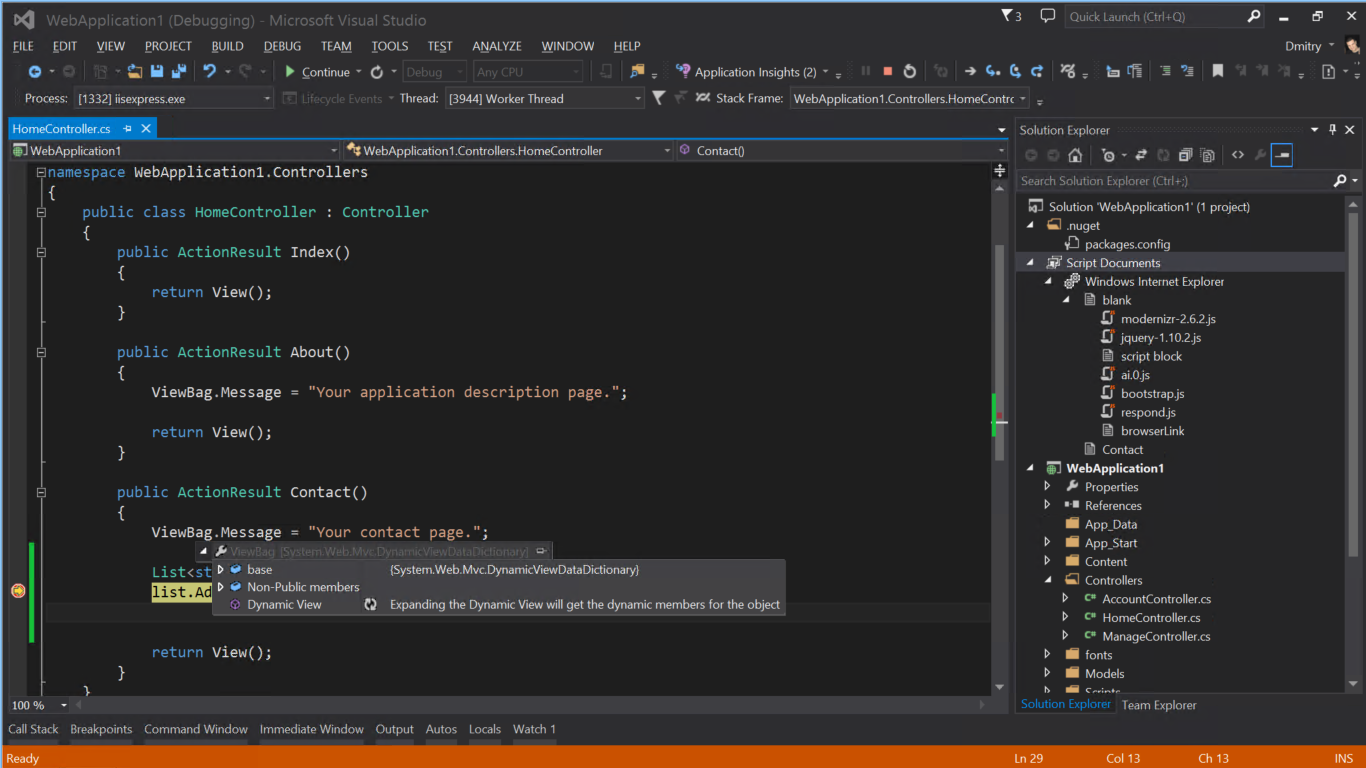
\includegraphics[width=0.5\paperwidth]{vscommunity}
\end{figure}

\subsection{Visual Studio Code + Terminal [Mac y Linux]}
El programa de Visual Studio Code es muy popular para la programación, tiene soporte para todos los lenguajes y es completamente gratis, con la desventaja de que no se puede compilar código.

Si estas en Windows, puedes utilizar este programa pero debes instalar algun emulador de terminal de sistemas Unix, como mingw para compilar código.

Si estas usando Mac o Linux, puedes compilar un programa de C++ desde la terminal. Para hacer esto, debe asegurar de tener instalado el paquete $gcc$ y debe generar un archivo ejecutable a partir del codigo con el comando $c++$

\begin{figure}[H]
    \centering
    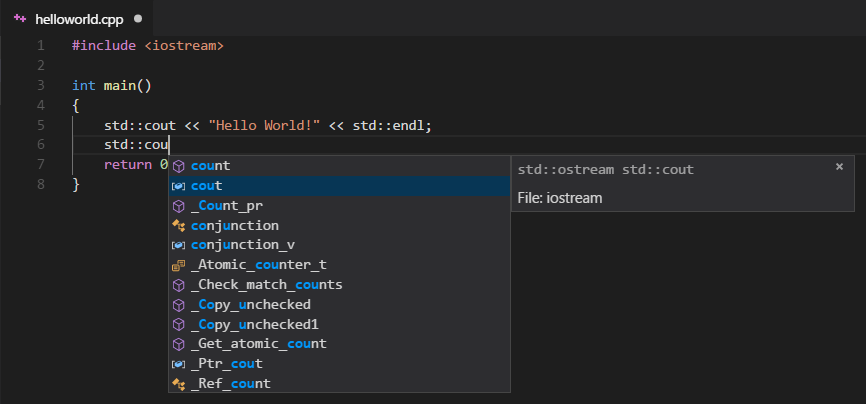
\includegraphics[width=0.5\paperwidth]{vscode}
\end{figure}

\section{Mi primer programa?}

\section{Leyendo y escribiendo}

\section{Errores comunes}

\subsection{Falta de inicialización}
Este error es uno de los mas graves y mas dificiles de detectar debido a que la lógica puede estar completamente correcta, el programa se compila sin errores y en algunos casos tus variables te podran dar los resultados correctos.

Esto pasa cuando defines una variable pero no le das un valor inicial. Por ejemplo:

\begin{lstlisting}[language=C++, caption=Error de inicialización]
#include <iostream>

using namespace std;

int main() {
    int i = 1;
    int suma;
    while(i <= 100) {
        suma += i;
        i++;
    }
    cout << suma << endl;
}
\end{lstlisting}

Este programa suma los numeros de 1 a 100 y los va guardando en la variable suma. Se esperaria que el resultado fuera 5050, pero si lo corres te despliega -1428474. Si vuelves a correr el codigo, ahora ves 82934. Este valor siempre cambia.

Esto ocurre debido a que nunca inicializamos o le damos un valor inicial a la variable suma. A la hora de declarar la variable, le estamos asegurando un espacio en la memoria del sistema pero esto no significa que ese espacio tenga guardado un cero. Puede ser que algun proceso anterior haya tenido que usar ese espacio y que haya dejado un valor que no nos interesa ahi.

La razon por la que siempre cambia es porque la memoria siempre esta siendo utilizado por otros procesos (Google Chrome, Word, etc.) y cada vez que corre el programa agarrara el primer espacio libre que encuentra para la variable suma, que no siempre será la misma.

Ahora existe una posibilidad de que tu compilador automaticamente detecte que suma no fue inicializado y le asigna el valor de cero despues, asi que esto puede hacer que el programa funciona en tu computadora pero a la hora de probarlo en otra falla.

Entonces para asegurar que esto nunca pase, siempre debes de tener la costumbre de inicializar tus variables a menos de que seran sobreescritos por otro valor o leidos desde la consola usando $cin$.

\subsection{Ciclos con otras variables}
Este error pasa muy seguido cuando se utilizan ciclos for anidados y cuando uno olvida que haya declarado una variable antes.

Digamos que vas tan mal en matematicas que se te olvidaron las tablas multiplicativas completamente, y tu quieres crear un programa que los genera. Puedes hacer esto con dos ciclos for, uno que calcule las filas y otra que calcule las columnas multiplicando los indices.

\begin{lstlisting}[language=C++, caption=Ciclos con otras variables]
#include <iostream>

using namespace std;

int main() {
    for(int i = 0; i <= 12; i++) {
        for(int j = 0; i <= 12; i++) {
            cout << i * j << "\t";
        }
        cout << endl;
    }
}
\end{lstlisting}

Al parecer este código esta bien, pero si miras fijamente veras que en el segundo ciclo estamos modificando i en lugar de j. El compilador asume que sabes lo que estas haciendo, asi que no te arroja ningun error al tener distintos variables en un solo ciclo.

Para asegurar que esto no pase, siempre debes asegurarte de que solo modifiques una variable por ciclo y que no habias usado esa variable antes.

\subsection{Error por uno}
Este error tiende a ser muy facil de arreglar y ocurre por fallas de logica.

Digamos que quieres encontrar la suma de todos los cuadrados $1^2 + 2^2 + 3^2 ... + n^2$, y creas un programa para hacer eso mismo.

\begin{lstlisting}[language=C++, caption=Error por uno]
#include <iostream>

using namespace std;

int main() {
    int n;
    cin >> n;
    int suma = 0;
    for(int i = 0; i < n; i++) {
        suma += i * i;
    }
    cout << suma << endl;
}
\end{lstlisting}

Corres tu programa con $n = 3$, y ya sabes que $1^2 + 2^2 + 3^2 = 1 + 4 + 9 = 14$, pero te dice que es 5. Ahora corres tu programa con $n = 4$ y ahora observas que la respuesta es 14 cuando debia ser 30. Esto ocurre porque estas contando de $0$ a $n-1$ (nota que el for tiene la expresión i < n cuando debia ser i <= n).

Esto pasó porque el for loop cuenta hasta n pero no lo incluye en la suma, y estos tipos de errores suelen ocurrir cuando se calculan valores que inician desde 1 o cuando deben incluir el ultimo valor.

\subsection{Segmentation fault}
Este error es algo común y suele pasar cuando quieres sacar un valor que esta fuera de un arreglo.

Digamos que tenemos un codigo que le pregunta al usuario un valor y luego despliega el factorial de ese valor. El código asume que el usuario seleccionará un numero entre 0 y 10, para luego desplegar su factorial el cual esta guardado en un arreglo.

\begin{lstlisting}[language=C++, caption=Error de inicialización]
#include <iostream>

using namespace std;

int main() {
    int factoriales[] = {1, 1, 2, 6, 24, 120, 720, 5040, 40320, 362880, 3628800};
    cout << "Que factorial quisieras?" << endl;
    int deseado;
    cin >> deseado;
    if(deseado < 0) {
        cout << "No existe " << deseado << "!";
    } else {
        cout << deseado << "! es " << factoriales[deseado] << endl;
    }
}
\end{lstlisting}

Ahora que pasa si el usuario quiere saber el valor de 25565 factorial? Si ejecutas el codigo con tal valor veras que el programa se cierra inesperadamente y regresa el siguiente error: [1] 12937 segmentation fault (core dumped).

Esto ocurre obviamente porque estas intentando accesar el elemento 25565 de un arreglo que solo tiene 10 valores, lo que pasa es que estas intentando ver un lugar que no existe en la memoria de tu programa.

El 95\% de las veces que veras un segmentation fault, será porque estas intentando modificar o ver un valor que esta fuera de un arreglo. Siempre debes asegurarte que un arreglo tiene suficiente espacio para guardar todos los posibles valores que ocupes.

\subsection{Sobreflujos}
Este error pasa cuando tienes un valor que es demasiado grande para una variable.

Ahora vamos a mejorar el codigo que habiamos hecho del factorial. En lugar de guardar los primeros 10 valores en un arreglo, vamos a generar cada valor con un ciclo.

Para checar que todo este bien, voy a desplegar los primeros 18 factoriales.

\begin{lstlisting}[language=C++, caption=Sobreflujo]
#include <iostream>

using namespace std;

int main() {
    int factorial = 1;
    for(int i = 1; i < 18; i++) {
        factorial *= i;
        cout << factorial << endl;
    }
}
\end{lstlisting}

Corres este codigo y te topas con una sorpresa, 17! es aparentemente -288522240. ¿Como fue que un factorial te dio un numero negativo si siempre incrementa?

Lo que esta pasando es que el valor de 17! es demasiado grande para guardar en un valor de tipo int, si buscas en linea encontraras que un int solo puede guardar valores de -2,147,483,648 a 2,147,483,647, y 17! tiene un valor de 355,687,428,096,000.

El programa no te arroja ningun error, simplemente lo que hace es que cuando un número es mas grande del valor maximo de 2,147,483,647, se traslapa a -2,147,483,648 y sigue sumando desde ese valor. Eso significa que si quiero guardo el valor de 2,147,483,649 en un int, me guardara en realidad -2,147,483,647.

Si sigues imprimiendo mas números, veras que se vuelven a hacer positivos y negativos debido a este traslape.

Para solucionar esto, debes reemplazar int por otro tipo de dato que pueda guardar numeros mas grandes, como long long int o double.

\subsection{Errores de redondeo}
Este error pasa cuando se dividen dos enteros.

Sabes que $\frac{1}{2} + \frac{1}{4} + \frac{1}{8} + \frac{1}{16} + ... = 1$ y quisieras comprobarlo creando un programa. Lo implementas con el siguiente codigo:

\begin{lstlisting}[language=C++, caption=Error de redondeo]
#include <iostream>

using namespace std;

int main() {
    int suma = 0;
    int potencia = 2;
    for(int i = 1; i < 30; i++) {
        suma += 1 / potencia;
        potencia *= 2;
    }
    cout << suma << endl;
}
\end{lstlisting}

Pero cuando lo corres, te dice que tu suma es cero. Revisas la variable de potencia y te das cuenta que esta bien, pero la variable se suma se queda en cero.

Esto ocurre debido a que 1 y potencia estan siendo guardados como enteros, y cuando se dividen dos enteros el resultado siempre sera otro entero redondeado para abajo. Es decir si hago $5 / 2$, esto me dara $2$ porque el valor de $2.5$ fue redondeado para abajo. Como potencia siempre es mayor que 1, esta division siempre se redondeara para abajo y dará cero.

Para corregir esto, se debe cambiar la variables de potencia y de suma de enteros a un tipo de dato flotante, es decir un número que permite puntos decimales.

\subsection{Faltas de memoria}
Esto sucede cuando tu programa ocupa demasiado espacio continuo y ocasiona un error.

A veces sucede que tienes que crear un arreglo con 10 millones de valores (es verdad, si vas a ocupar algo asi!) y te das cuenta que tu programa deja de funcionar.

\begin{lstlisting}[language=C++, caption=Faltas de memoria]
#include <iostream>

using namespace std;

int main() {
    int arreglo[10000000];
    for(int i = 0; i < 10000000; i++) {
        arreglo[i] = i;
    }
    cout << "Arreglo llenado" << endl;
}
\end{lstlisting}

Por suerte, esto se puede arreglar. Si cuentas los bytes, te daras cuenta que son 4 millones de bytes o 4 megabytes, y computadoras modernas tienden a tener hasta 16 gigabytes de espacio, asi que no debe haber problema para conseguir 4 megabytes de memoria.

El problema viene del hecho que a la hora de crear un arreglo, el sistema busca 4 megabytes de espacio que esten libres y juntos dentro de la memoria del programa. Esto se puede arreglar preguntandole a tu sistema si puedes guardar estos 4 megabytes en una area especial extra de memoria llamado el heap, que viene siendo una area publica con muchisimo espacio, en lugar del espacio limitado que fue asignado a tu programa.

Para hacer que el programa busque dentro del heap, debes cambiar el arreglo a un puntero y utilizar malloc, new o alguna funcion que te permite obtener espacio del heap.

\section{Tipos de datos}

\subsection{Signed y unsigned}

\subsection{Numericos}

\subsection{Caracteres y cadenas}

\subsection{Booleanos}

\subsection{Long long}

\subsection{Arreglos}

\section{Funciones}

\end{document}

